\let\negmedspace\undefined
\let\negthickspace\undefined
\documentclass[journal]{IEEEtran}
\setlength{\headheight}{1cm} % Set the height of the header box
\setlength{\headsep}{0mm}     % Set the distance between the header box and the top of the text
\usepackage[a4paper,margin=10mm, onecolumn]{geometry}
\usepackage{gvv-book}
\usepackage{gvv}
\usepackage{cite}
\usepackage{amsmath,amssymb,amsfonts,amsthm}
\usepackage{algorithmic}
\usepackage{graphicx}
\usepackage{textcomp}
\usepackage{xcolor}
\usepackage{txfonts}
\usepackage{listings}
\usepackage{enumitem}
\usepackage{mathtools}
\usepackage{gensymb}
\usepackage{comment}
\usepackage[breaklinks=true]{hyperref}
\usepackage{tkz-euclide}
\usepackage{listings}
\def\inputGnumericTable{}
\usepackage[latin1]{inputenc}
\usepackage{color}
\usepackage{array}
\usepackage{longtable}
\usepackage{calc}
\usepackage{multirow}
\usepackage{hhline}
\usepackage{ifthen}
\usepackage{lscape}
\usepackage{circuitikz}
\tikzstyle{block} = [rectangle, draw, fill=blue!20,
    text width=4em, text centered, rounded corners, minimum height=3em]
\tikzstyle{sum} = [draw, fill=blue!10, circle, minimum size=1cm, node distance=1.5cm]
\tikzstyle{input} = [coordinate]
\tikzstyle{output} = [coordinate]
\begin{document}
\bibliographystyle{IEEEtran}
\vspace{3cm}
\title{3.2.29}
\author{AI25BTECH11013-Gautham}
\maketitle
% \newpage
% \bigskip
{\let\newpage\relax\maketitle}
\renewcommand{\thefigure}{\theenumi}
\renewcommand{\thetable}{\theenumi}
\setlength{\intextsep}{10pt} % Space between text and floats
\numberwithin{equation}{enumi}
\numberwithin{figure}{enumi}
\renewcommand{\thetable}{\theenumi}
\textbf{Question}:\\
Construct a $\triangle ABC$ given 
\begin{align}
a = BC = 6\ \text{cm},\qquad \angle B = 30^\circ,\qquad AC - AB = 4\ \text{cm}.\\
\end{align}

\solution \\
In the usual notation $a=BC,\; b=CA,\; c=AB$.  From the cosine formula in $\triangle ABC$\\
\begin{align}
b^2 = a^2 + c^2 - 2ac\cos B. 
\end{align}
Put $b = c + k$ where $k = 4$. 
\begin{align}
(c+k)^2 = a^2 + c^2 - 2ac\cos B.
\end{align}
Canceling $c^2$ and collecting terms in $c$:
\begin{align}
2kc + k^2 = a^2 - 2ac\cos B
\quad\Longrightarrow\quad
c\big(2k + 2a\cos B\big) = a^2 - k^2.
\end{align}
Hence the general expression for $c$ when $b-c=k$ is
\begin{equation}
\boxed{\, c \;=\; \frac{a^2 - k^2}{2\,(k + a\cos B)} \,}. \label{eq:c_general}
\end{equation}

Now substitute $a=6,\; B=30^\circ,\; k=4$:
\begin{align}
\cos 30^\circ = \frac{\sqrt3}{2},\qquad
c = \frac{6^2 - 4^2}{2\big(4 + 6\cos 30^\circ\big)}
= \frac{36 - 16}{2\big(4 + 6\cdot\frac{\sqrt3}{2}\big)}
= \frac{20}{2\big(4 + 3\sqrt3\big)}.
\end{align}
Numerically,
\begin{align}
c \approx 1.09\ \text{cm},\qquad b = c + 4 \approx 5.09\ \text{cm}.
\end{align}

Place $\Vec{B}=\myvec{0 \\ 0}$ and $\Vec{C}=\myvec{a \\ 0}=\myvec{6 \\ 0}$.
Point $A$ lies on this ray with $BA=c$, so
\begin{align}
\Vec{A}=c\myvec{\cos B \\ \sin B}
\approx (0.94, 0.54).
\end{align}
\begin{figure}[h!]
    \centering
    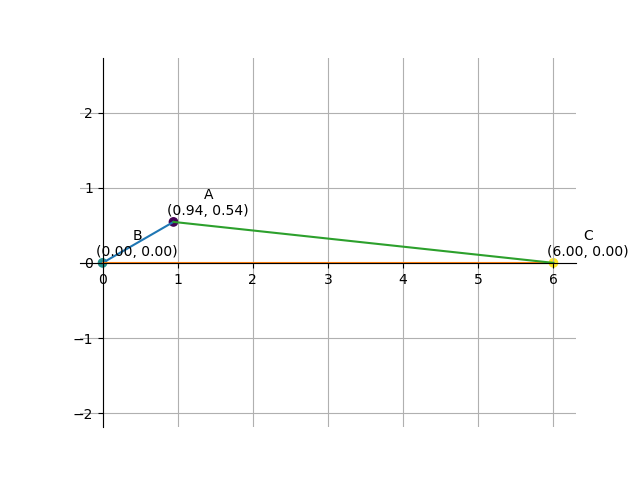
\includegraphics[height=0.6\textheight, keepaspectratio]{figs/fig.png}
    \label{figure_1}
\end{figure}


\end{document}
